\section{Background}
\label{intro}

Deception is a routine part of human communication, and the shift of everyday interaction onto digital platforms has not reduced it -- if anything, textual computer-mediated communication (\gls{cmc}) has made deception cheaper to produce and harder to detect, because the visual and vocal cues that people rely on in face-to-face settings (facial expression, vocal pitch, gaze) are simply absent from text \cite{zhou2003exploratory}. Fabricated product reviews, phishing messages, fraudulent job postings, misleading political statements, and fake news articles are all instances of the same underlying problem: a writer choosing to misrepresent the truth in text, and a reader (or an automated system standing in for the reader) needing to tell the misrepresentation apart from a truthful message using nothing but the words themselves.
\begin{table}[htbp]
\centering
\caption{Illustrative examples of deception detection using the proposed system.}
\label{tab:prediction_example}
\renewcommand{\arraystretch}{1.3}
\begin{tabular}{|p{7.0cm}|c|c|c|}
\hline
\textbf{Input Text} &
\textbf{Category} &
\textbf{Language} &
\textbf{Prediction} \\
\hline

Click here to verify your bank account immediately. &
Phishing &
English &
Deceptive \\
\hline

{\bengali আপনার ব্যাংক অ্যাকাউন্ট যাচাই করতে এখনই এই লিংকে ক্লিক করুন।} &
Phishing &
Bangla &
Deceptive \\
\hline

Apnar bank account verify korte ekhuni ei link e click korun. &
Phishing &
Banglish &
Deceptive \\
\hline

This product exceeded my expectations. &
Review &
English &
Truthful \\
\hline

{\bengali এই পণ্যটি আমার প্রত্যাশার চেয়েও ভালো ছিল।} &
Review &
Bangla &
Truthful \\
\hline

Ei product ta amar expectation er cheyeo valo chilo. &
Review &
Banglish &
Truthful \\
\hline

\end{tabular}
\end{table}
Early computational approaches to this problem relied on hand-crafted linguistic cues -- lexical diversity, sentiment, pronoun usage, and similar surface statistics -- combined with classical machine learning classifiers \cite{zhou2003exploratory}. More recent work has moved toward deep contextual language models, particularly Transformer-based encoders such as \gls{bert} \cite{devlin2019bert}, which learn distributed representations of text directly from large corpora and have substantially improved deception- and misinformation-detection accuracy across domains such as courtroom testimony, hotel reviews, and social media posts \cite{fornaciari2021bertective, ilias2022explainable}. In parallel, the fake-news-detection literature has explored architectures ranging from multimodal attention networks that fuse gaze and speech signals \cite{gallardo2021detecting} to convolutional Transformer hybrids for social-media content \cite{djenouri2024federated} and large-language-model-based transfer learning pipelines \cite{alqadi2025transfer}.

Two practical obstacles, however, limit how much of this progress transfers to a setting such as Bangladesh, and more broadly to any multilingual, privacy-sensitive population. First, almost all of the datasets and pretrained models above are English-centric; a deceptive message written in Bangla, or in the Romanized Bangla ("Banglish") that is extremely common in everyday Bangladeshi digital communication, is poorly served by models trained only on English text. Second, and just as importantly, the data needed to train a strong deception detector -- private product reviews, personal job applications, political opinions, suspicious messages people have received -- is exactly the kind of data that individuals and organizations are reluctant to centralize on a single server for training, both for privacy reasons and, increasingly, because of regulatory constraints on data movement. A deception-detection system that requires pooling everyone's raw text in one place is therefore difficult to deploy in practice, however accurate it may be in a benchmark setting.

\section{Motivation}

Federated learning (\gls{fl}) offers a direct answer to the second obstacle. Instead of moving data to a central server, \gls{fl} moves a model out to where the data already lives, trains it locally, and only ever communicates model updates -- never raw text -- back to a coordinating server \cite{mcmahan2017communication}. This makes it structurally compatible with realistic deployment scenarios in which a fake-news detector, a phishing filter, a review-authenticity checker, a job-scam flagger, and a political-statement fact-checker might each be operated by a different organization that cannot or will not share its raw data with the others, yet all five would benefit from a shared underlying language understanding of what deceptive text tends to look like. Related work has already shown that federated fake-news detectors can approach the accuracy of centrally-trained ones while keeping user data local \cite{lian2024find, marulli2021exploring}, but this line of work has so far been evaluated mostly on English, single-domain, and often synthetically-partitioned data, leaving open how well the same idea holds up under a harder, more realistic form of heterogeneity: multiple languages, multiple deception domains, and a strict non-overlapping partition of clients by domain rather than by convenience.
\begin{figure}[htbp]
    \centering
    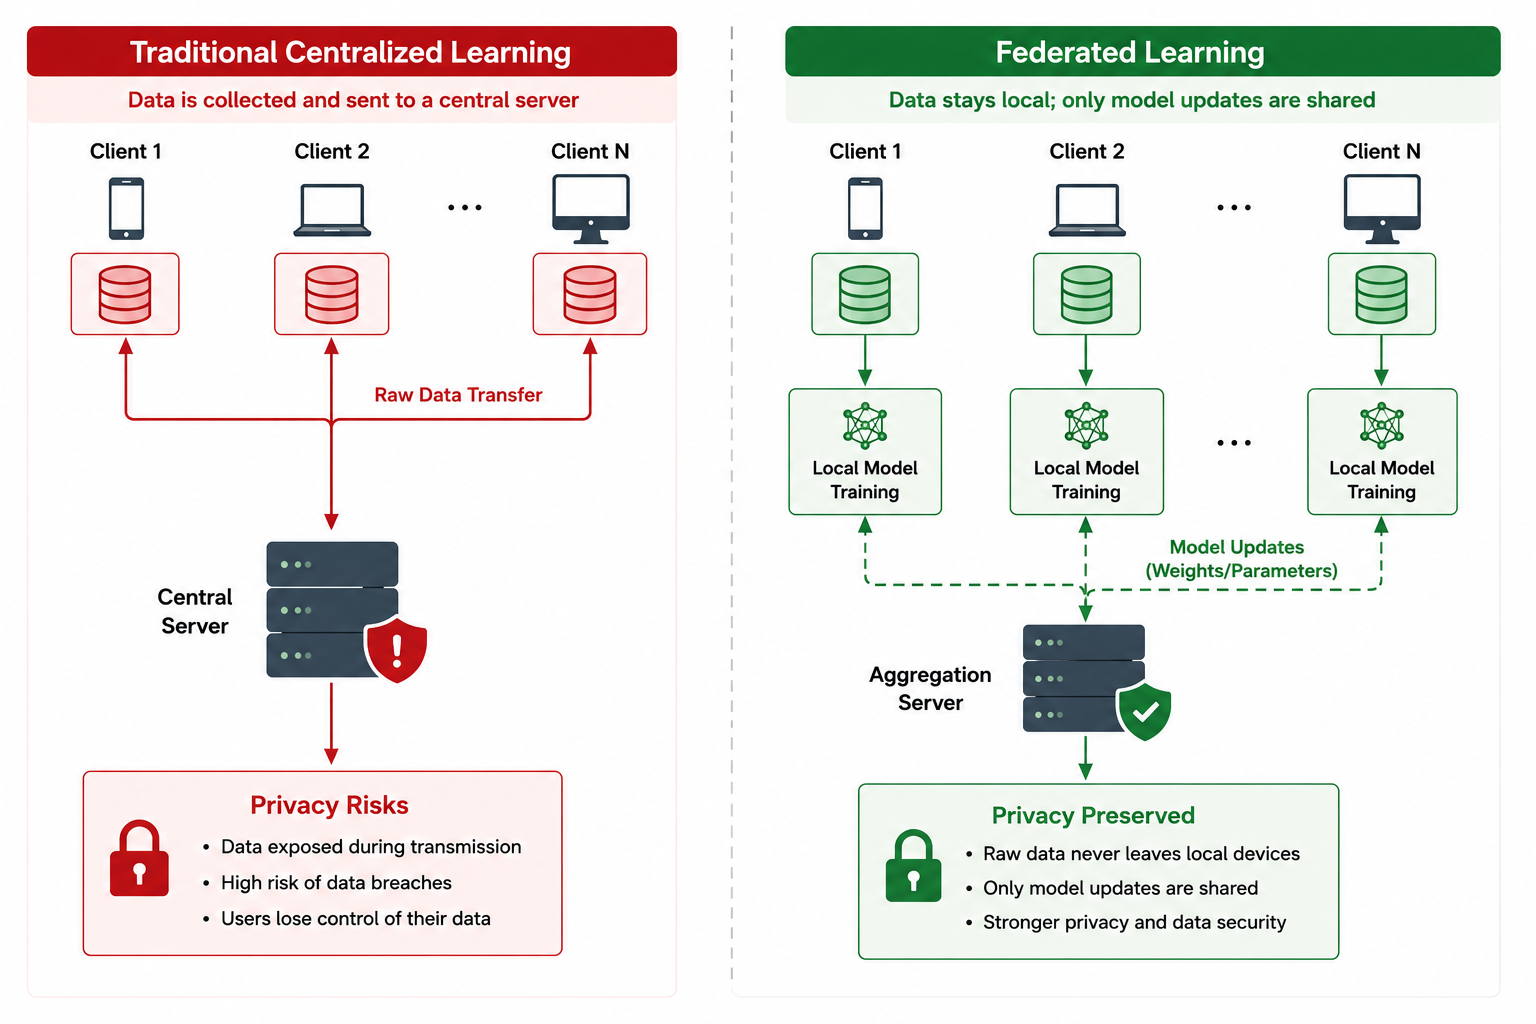
\includegraphics[width=0.95\textwidth]{figures/Introduction_image.png}
    \caption{Comparison between traditional centralized learning and privacy-preserving federated learning.}
    \label{fig:intro-fl-comparison}
\end{figure}
At the same time, the handful of studies that specifically target Bangla text classification with Transformer encoders \cite{abdal2023transformer} confirm that multilingual and Bangla-specific pretrained encoders (such as \gls{mbert}, \gls{xlmr}, \gls{muril}, and BanglishBERT) are viable for downstream classification, but none of them combine this multilingual capability with a federated, privacy-preserving training regime, and none of them study deception detection specifically across several distinct deception domains at once. This thesis is motivated by that gap: the need for a deception detection system that (i) works across English, Bangla, and Banglish text within a single unified model, (ii) covers multiple deception domains rather than a single narrow task, and (iii) is trainable without centralizing any client's raw data, using a federated optimization strategy robust enough to handle the resulting statistical heterogeneity.

\section{Problem Statement}

Formally, the problem addressed in this thesis is binary text classification: given a short piece of text, predict whether it is deceptive or truthful (\texttt{is\_deceptive} $\in \{0,1\}$). What makes the problem non-trivial in this setting is threefold:

\begin{itemize}
    \item \textbf{Multilinguality.} The input text may be in English, Bangla, or Banglish (Bangla transliterated into Roman script), and the model must handle all three registers without being told in advance which one it is looking at.
    \item \textbf{Multi-domain, non-\gls{fl}-friendly heterogeneity.} The data spans five deception domains -- fake news, product reviews, phishing, political statements, and job scams -- and in the federated setting each domain is held by a single client with zero overlap with the others. This is a considerably more extreme form of non-\gls{fl} data heterogeneity than the typical federated learning benchmark, where each client usually holds a random, class-balanced subsample of a single task.
    \item \textbf{Privacy constraint.} No client may transmit its raw text to the server or to any other client; only model parameters (or updates derived from them) may be communicated, and the aggregation strategy must remain robust to client drift under the heterogeneity described above.
\end{itemize}

\section{Objectives of the Thesis}

The specific objectives of this work are to:
\begin{enumerate}
    \item Construct a multilingual (English / Bangla / Banglish), multi-domain deception detection dataset by stratified sampling and translation/transliteration of the Generalized Deception Dataset \cite{zeng2022generalized}, preserving class balance and domain distribution.
    \item Design a single attention-pooling classification architecture that can sit on top of several different multilingual pretrained encoder backbones (\gls{mbert} \cite{devlin2019bert}, \gls{xlmr} \cite{conneau2020xlmr}, \gls{muril} \cite{khanuja2021muril}, BanglishBERT \cite{bhattacharjee2022banglabert}, and a distilled multilingual \gls{albert} variant \cite{lan2020albert}) without changing the classification head.
    \item Establish a centralized (non-federated) accuracy baseline for each backbone on the pooled training data.
    \item Implement a realistic cross-domain federated learning pipeline using the Flower framework \cite{beutel2020flower} with the \gls{fedprox} optimization strategy \cite{li2020federated}, treating each deception domain as one federated client, and compare its performance against the centralized baseline for the same backbones.
    \item Analyze the accuracy-retention (federated performance relative to centralized performance for the same backbone) as the primary diagnostic of the privacy-utility trade-off, rather than relying on raw accuracy alone, since raw accuracy comparisons across different backbones or training paradigms can be misleading.
\end{enumerate}

\section{Contribution of the Thesis}

The main contributions of this thesis are:

\begin{enumerate}
    \item A multilingual, multi-domain deception detection benchmark built from a stratified, class-balanced sample of the Generalized Deception Dataset \cite{zeng2022generalized}, mixed across English (60\%), Bangla (30\%), and Banglish (10\%) registers, spanning five deception domains.
    \item An attention-pooling classification architecture, decoupled from the choice of encoder backbone, allowing a like-for-like comparison of five multilingual/Bangla-aware encoders under identical training conditions.
    \item A realistic, extreme non-\gls{fl}-friendly federated learning benchmark in which each of the five deception domains is assigned to exactly one client, evaluated using the \gls{fedprox} strategy \cite{li2020federated} rather than plain \gls{fedavg} \cite{mcmahan2017communication}, together with a same-backbone accuracy-retention analysis that isolates the true cost of federation from the cost of choosing a weaker encoder.
    \item An empirical comparison across five backbones and two training paradigms (centralized vs.\ federated), reported with accuracy, precision, recall, macro-F1, \gls{auc}, and \gls{mcc}, giving a more complete picture than accuracy alone, particularly given the class-imbalance risk inherent in domain-partitioned data.
\end{enumerate}

\section{Thesis Organization}

The remainder of this thesis is organized as follows. \Cref{chap:lr} reviews related work in deception and fake-news detection, multilingual/Bangla-aware Transformer encoders, and federated learning, and positions this thesis relative to that body of work. \Cref{chap:method} describes the dataset construction process, the attention-pooling classification architecture, the centralized training setup, and the \gls{fedprox}-based federated training pipeline, including the infrastructure used and the practical issues encountered during implementation. \Cref{chap:results} presents the experimental results for all five backbones under both training paradigms, along with the accuracy-retention analysis. \Cref{chap:conclusion} concludes the thesis and outlines directions for future work.

\section{Summary}

This chapter introduced the motivation for combining multilingual deception detection with privacy-preserving federated learning, stated the problem this thesis addresses, and outlined the objectives, contributions, and organization of the remaining chapters.
